It's no secret that as a project grows, it becomes harder and harder to find things in it – both in listfiles and in the source code. Therefore, it is very important to maintain the project hygiene right from the get-go.

Imagine a scenario where you need to deliver some important, time-sensitive changes, and they don't fit well in either of the two directories in your project. Now, you need to quickly push a cleanup commit that introduces more directories and another level of hierarchy for your files so that your changes can have a nice place to fit. Or (what's worse), you decide to just shove them anywhere and create a ticket to deal with the issue later.

Over the course of the year, these tickets accumulate, the technical debt grows, and so does the cost of maintaining the code. This becomes extremely troublesome when there's a crippling bug in a live system that needs a quick fix and when people unfamiliar with the code base need to introduce their changes.

So, we need a good project structure. But what does this mean? There are a few rules that we can borrow from other areas of software development (for example, system design).
The project should have the following characteristics:

\begin{itemize}
\item 
It should be easy to navigate and extend

\item 
It should be self-contained – for example, project-specific files should be in the project directory and nowhere else.

\item 
The abstraction hierarchy should be expressed through executables and binaries.
\end{itemize}

There is no single agreed-upon solution, but among the many available project structure templates online, I recommend following this one, as it is simple and very extensible:

\begin{center}
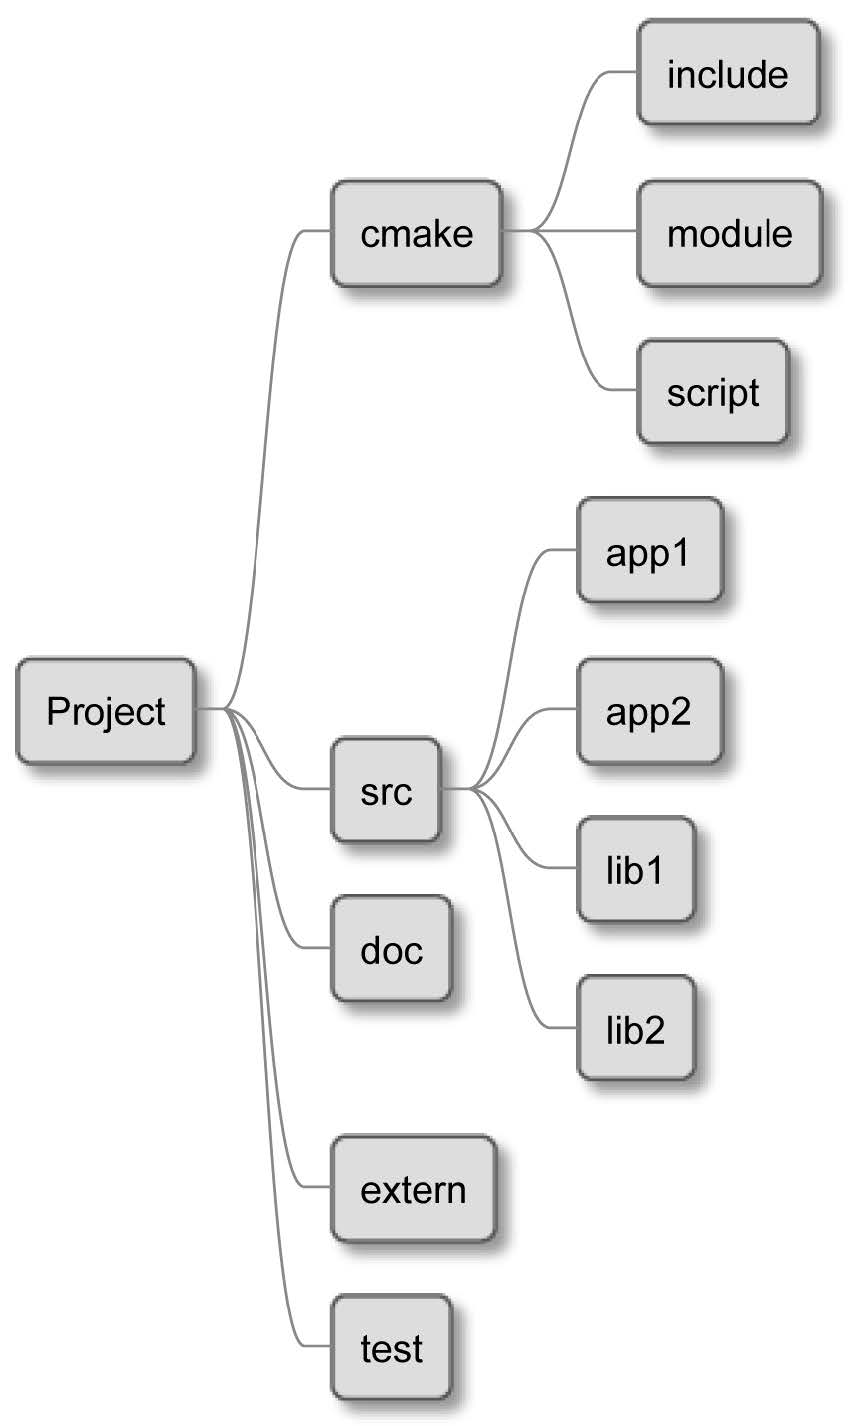
\includegraphics[width=0.8\textwidth]{content/1/chapter3/images/1.jpg}\\
Figure 3.1 – An example of a project structure
\end{center}

This project outlines the directories for the following components:

\begin{itemize}
\item 
cmake: Includes macros and functions, find\_modules, and one-off scripts

\item 
src: Will store the source of our binaries and libraries

\item 
doc: Used for building the documentation

\item 
extern: Configuration for the external projects we are building from source

\item 
test: Contains code for automated tests
\end{itemize}

In this structure, the CMakeLists.txt file should exist in the following directories: the top-level project directory, src, doc, extern, and test. The main listfile shouldn't declare any build steps on its own, but instead, it should use the add\_subdirectory() command to execute all of the listfiles in the nested directories. In turn, these may delegate this work to even deeper layers if needed.

\begin{tcolorbox}[colback=blue!5!white,colframe=blue!75!black,title=Note]
Some developers suggest separating the executables from the libraries and creating two top-level directories instead of one: src and lib. CMake treats both artifacts the same, and separation at this level doesn't really matter.
\end{tcolorbox}

Having multiple directories in the src directory comes in handy for bigger projects. But if you're building just a single executable or library, you may skip them and store your source files directly in src. In any case, remember to add a CMakeLists.txt file there and execute any nested listfiles as well.

This is how your file tree might look for a single target:

\begin{center}
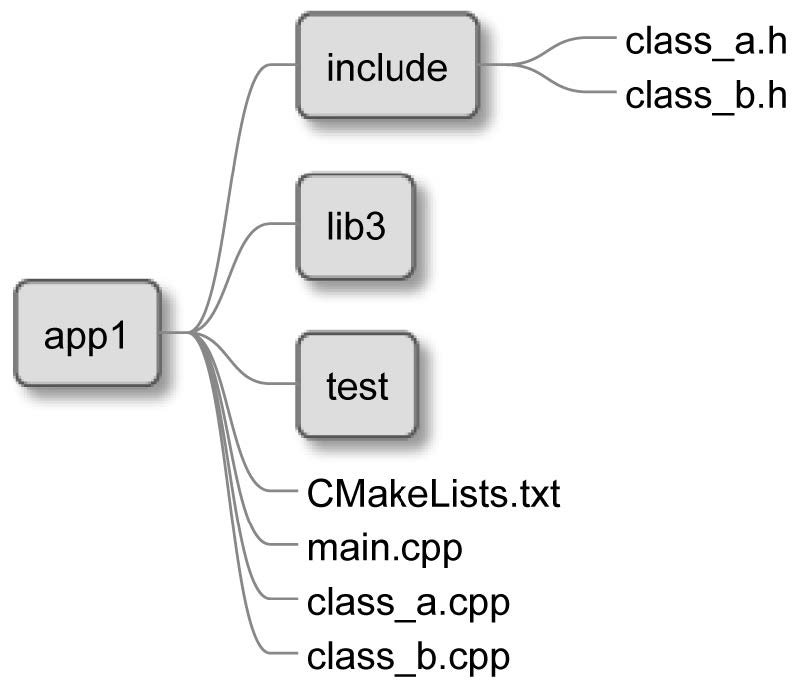
\includegraphics[width=0.8\textwidth]{content/1/chapter3/images/2.jpg}\\
Figure 3.2 – The directory structure of an executable
\end{center}

We see a CMakeLists.txt file in the root of the app1 directory – it will configure the key project settings and include all listfiles from nested directories. The src directory contains another CMakeLists.txt file along with the .cpp implementation files: two classes and the main file with the executable's entry point. The CMakeLists.txt file should define a target that uses these sources to build an executable – we'll learn how to do that in the next chapter.

Our header files go to the include directory – these are used by .cpp implementation files to declare symbols from other C++ translation units.

We have a test directory to store the source code for our automated tests, and we also have lib3, which contains a library specific to this executable only (libraries used elsewhere in the project or exported outside of it should live in the src directory).

This structure is pretty expressive and allows for many extensions of the project. As we keep adding more and more classes, we can easily group them in libraries to speed up the compilation process. Let's see what a library looks like:

\begin{center}
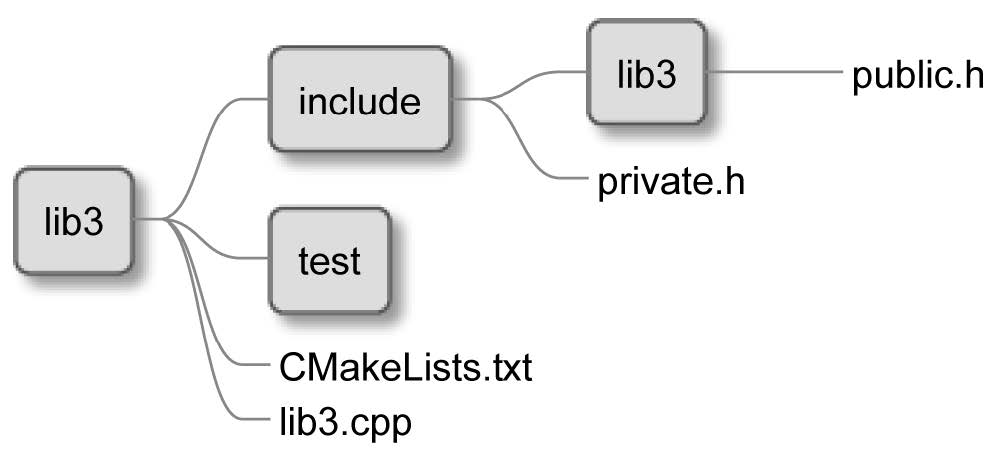
\includegraphics[width=0.8\textwidth]{content/1/chapter3/images/3.jpg}\\
Figure 3.3 – The directory structure of a library
\end{center}

As it turns out, libraries follow the same structure as executables, with only a small difference: there is an optional lib3 directory in the include directory. This should only be present if we use the library externally from the project. It provides the public header files that other projects will consume during compilation. We'll return to this subject when we start building our own libraries in Chapter 5, Compiling C++ Sources with CMake.

So, we have discussed how files are laid out in a directory structure. Now, it's time to take a look at how individual CMakeFiles.txt files come together to form a single project and what their role is in a bigger scenario.

\begin{center}
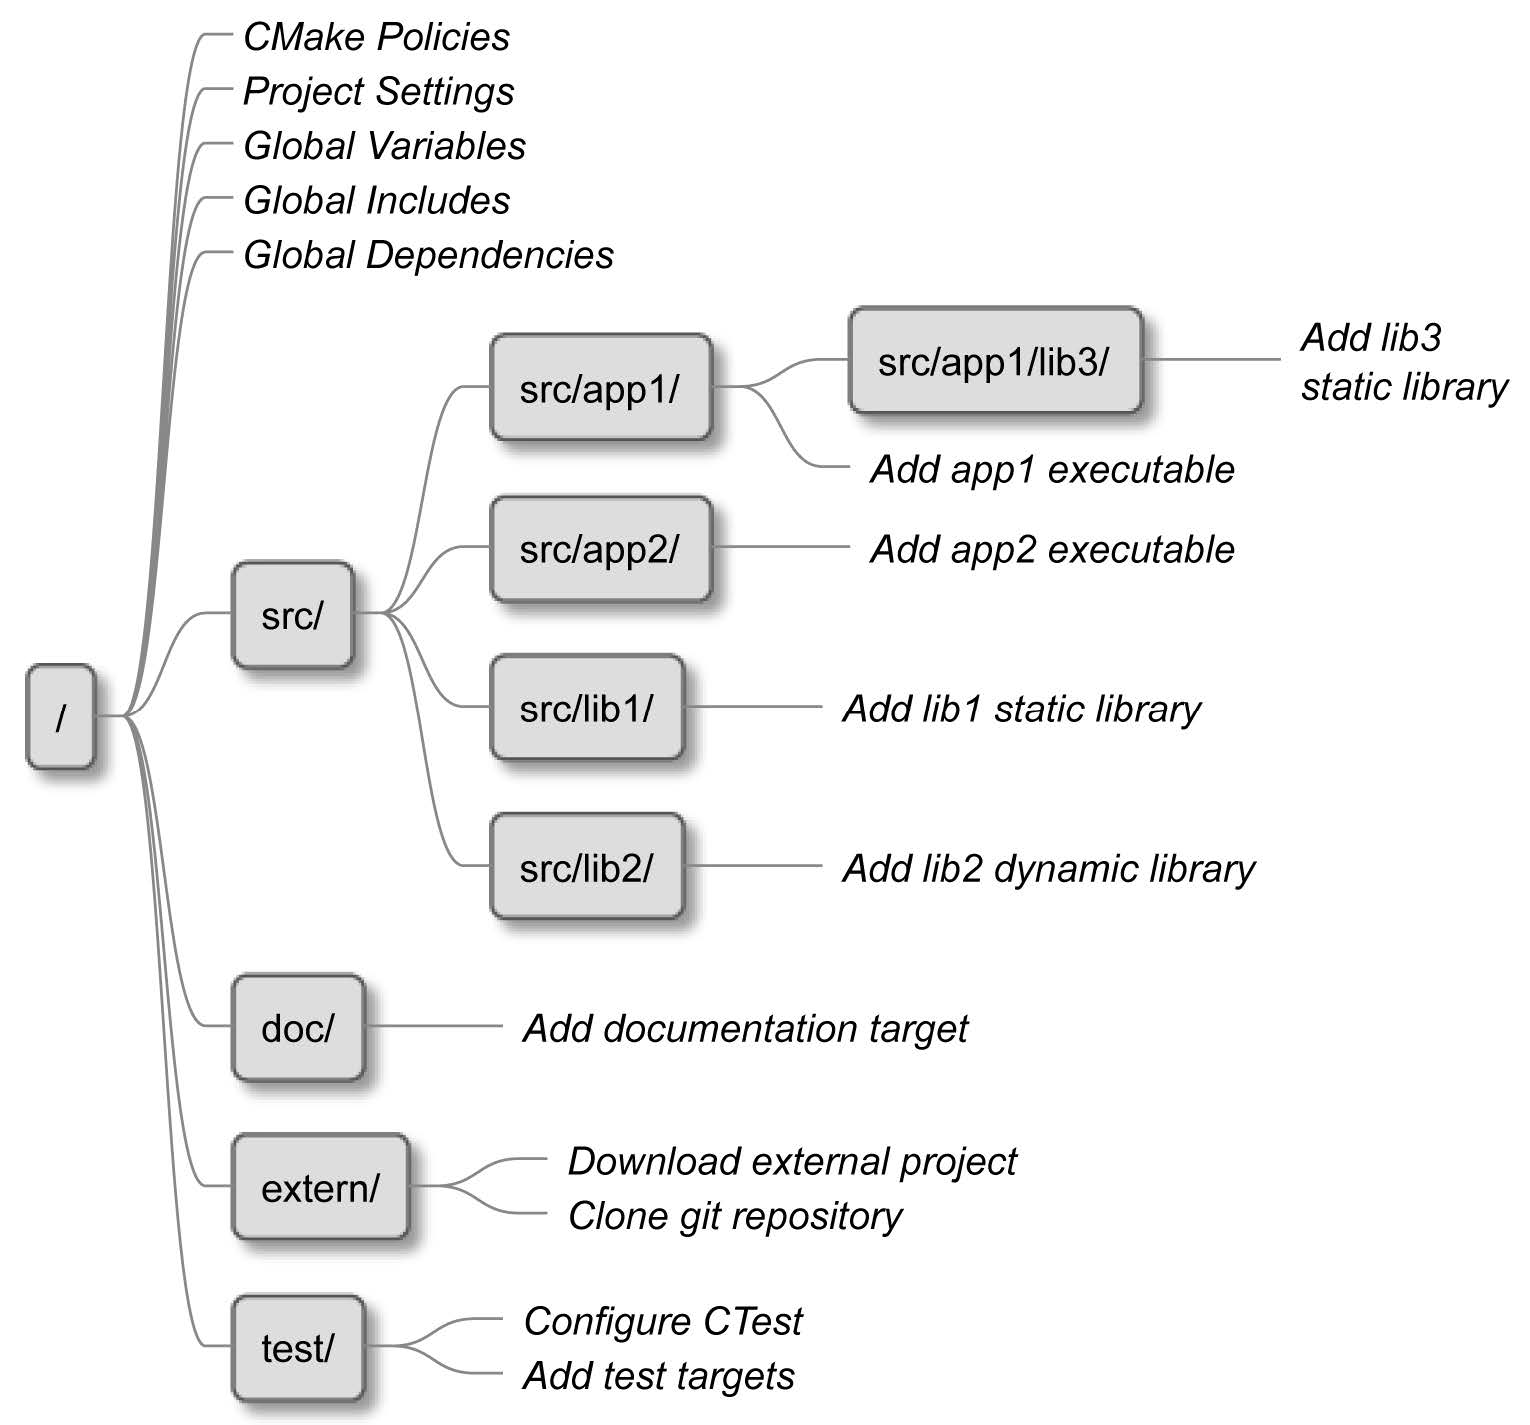
\includegraphics[width=0.8\textwidth]{content/1/chapter3/images/4.jpg}\\
Figure 3.4 – How CMake merges listfiles together in a single project
\end{center}

In Figure 3.4, each box represents a CMakeLists.txt listfile residing in a given directory, while the labels in cursive text represent the actions executed by each file (from top to bottom). Let's analyze this project once more from CMake's perspective:

\begin{enumerate}
\item 
The execution starts from the root of the project – that is, from a listfile residing in the source tree. This file will set the minimum required CMake version with the appropriate policies, set the project name, supported languages, global variables, and include the files from the cmake directory so that their contents are available globally.

\item 
The next step is to enter the scope of the src directory by calling the add\_subdirectory(src bin) command (we'd like to put compiled artifacts in <binary\_tree>/bin rather than <binary\_tree>/src).

\item 
CMake reads the src/CMakeLists.txt file and discovers that its only purpose is to add four nested subdirectories: app1, app2, lib1, and lib2.

\item 
CMake enters the variable scope of app1 and learns about another nested library, lib3, which has its own CMakeLists.txt file; then the scope of lib3 is entered.

\item 
The lib3 library adds a static library target with the same name. CMake returns to the parent scope of app1.

\item 
The app1 subdirectory adds an executable that depends on lib3. CMake returns to the parent scope of src.

\item 
CMake will continue entering the remaining nested scopes and executing their listfiles until all add\_subdirectory() invocations have been completed.

\item 
CMake returns to the top-level scope and executes three remaining commands: add\_subdirectory(doc), add\_subdirectory(extern), and add\_subdirectory(test). Each time, CMake enters the new scope and executes commands from the appropriate listfile.

\item 
All of the targets are collected and checked for their correctness. CMake now has all of the necessary information to generate a buildsystem.
\end{enumerate}

We need to remember that the preceding steps are happening in the exact order in which we wrote the commands in our listfiles. Sometimes this matters, while other times, not so much. We'll get to the bottom of that in the next chapter.

So, when is the right time to create the directories to contain all of the elements of the project? Should we do it right from the start – create everything needed for the future and keep the directories empty – or wait until we actually have the files that need to go in their own category? This is a choice – we could follow the extreme-programming rule YAGNI (you aren't gonna need it), or we could try to make our project future-proof and lay good foundations for new developers to come.

Try to aim for a good balance between these approaches – if you suspect that your project might one day need an extern directory, then add it (you may need to create an empty .keep file to check a directory into the repository). To help others know where to put their external dependencies, create a readme file, and lay the path for less experienced programmers who will travel this road in the future. You may have observed this yourself: developers are reluctant to create directories, especially in the root of the project. If we provide a good project structure, people will be inclined to follow it.

Some projects can be built in almost every environment, while others are quite particular about their specifics. The top-level listfile is the perfect place to assess how to proceed with the project, depending on what is available. Let's see how to do this.





